\documentclass[12pt, titlepage]{article}
\usepackage[shortlabels]{enumitem}
\usepackage{booktabs}
\usepackage{tabularx}
\usepackage{hyperref}
\usepackage{graphicx}
\usepackage{float}
\hypersetup{
    colorlinks,
    citecolor=black,
    filecolor=black,
    linkcolor=red,
    urlcolor=blue
}
\usepackage[round]{natbib}

\title{SE 3XA3: Test Plan\\GoDBMS}

\author{Team \#7, Databased
		\\ Faiq Ahmed, ahmedf46
		\\ Eesha Qureshi, qureshe
		\\ Kevin Kannammalil, kannammk
}

\date{March 11, 2022}

\begin{document}

\maketitle

\pagenumbering{roman}
\tableofcontents
\listoftables
\listoffigures

\begin{table}[H]
\caption{\bf Revision History}
\begin{tabularx}{\textwidth}{p{3cm}p{2cm}X}
\toprule {\bf Date} & {\bf Version} & {\bf Notes}\\
\midrule
March 9, 2022 & 1.0 & Initial Document \\
March 10, 2022 & 1.2 & Started Tests for Functional Requirements \\
March 10, 2022 & 1.2 & Finished Introduction \\
March 11, 2022 & 1.2 & Finished Functional Requirement Tests \\
March 11, 2022 & 1.2 & Finished Non-Functional Requirement Tests \\
March 11, 2022 & 1.3 & Final Draft \\
\bottomrule
\end{tabularx}
\end{table}

\newpage

\pagenumbering{arabic}

This document outlines the testing plan for the GoDBMS system.

\section{General Information}

\subsection{Purpose}
The purpose of this document is to provide in depth details of the testing plans and methods that will be used to verify the functionality of the GoDBMS software.

\subsection{Scope}
The test suites that comprise this document will be used to ensure that the software meets its functional and non-functional requirements that were outlined in the Software Requirements Specification (SRS). It will cover both the specific tests, as well as the testing tools and environments used to execute them. The tests will additionally cover verification procedures for the Proof of Concept (POC), as well as internal unit testing plans.

\subsection{Acronyms, Abbreviations, and Symbols}
	
\begin{table}[H]
\caption{\textbf{Table of Abbreviations}} \label{Table}

\begin{tabularx}{\textwidth}{p{3cm}X}
\toprule
\textbf{Abbreviation} & \textbf{Definition} \\
\midrule
SRS & Software Requirements Specification; a document that outlines important information about the software project such as stakeholders, functional requirements, non-functional requirements and project scope \\
POC & Proof of Concept; a prototype, demo or design that provides evidence of the project's feasibility \\
DBMS & \textbf{Database} Management System; software that allows a user to perform \textbf{database} transactions and operations\\
CLI & Command Line Interface; the point of communication between the software and the user \\
Go & GoLang \\
\bottomrule
\end{tabularx}

\end{table}

\begin{table}[!htbp]
\caption{\textbf{Table of Definitions}} \label{Table}

\begin{tabularx}{\textwidth}{p{3cm}X}
\toprule
\textbf{Term} & \textbf{Definition}\\
\midrule
\textbf{Database} & A set of \textbf{record}s that store information organized by keys\\
\textbf{Command Line} & The point of communication between user and internal computer instructions\\
\textbf{Table} & An organized collection of \textbf{record}s in a \textbf{database}\\
\textbf{Record} & A single row of data in a \textbf{database}\\
\textbf{Primary Key} & A unique identifier for a \textbf{record} in a \textbf{database}\\
\textbf{Struct} & A modular collection of fields in GoLang \\
\textbf{Schema} & An outline of fields, table names, and relationships in a \textbf{database} \\
\textbf{Columns} & Vertical aggregations of data in a table \\
\textbf{Catalog} & A list storing the names of all the tables in the database. This list can be encoded and decoded from a file to allow persistent storage.\\
\textbf{Tuple} & An immutable finite sequence of elements\\
\textbf{Message Passing} & The method of invoking a process in a computer\\
\textbf{Concurrency} & The use of threads to run multiple computer processes at the same time\\
\textbf{GoLang} & A compiled programming language\\

\bottomrule
\end{tabularx}

\end{table}	

\subsection{Overview of Document}
This document will outline the testing team and tools, test schedule, functional and non functional tests, POC testing, and unit testing.

\section{Plan}
	
\subsection{Software Description}

GoDBMS is a \textbf{database} management system based off of SimpleDB, which is an open source Java based DBMS. GoDBMS changes the implementation of this DBMS to be simpler and more focused on the \textbf{message passing} \textbf{concurrency} model of \textbf{Go} programming language to reduce the complexity of the design and improve its concurrent performance.

\subsection{Test Team}

The test team for this project consists of the members of the Databased group: Faiq Ahmed, Kevin Kannammalil, and Eesha Qureshi.\\

\noindent These members will be responsible for writing the test cases that encompass this project as the project is being developed, as well as create and distribute the necessary interviews and surveys needed to get feedback on the non functional requirements of this project.

\subsection{Automated Testing Approach}

Automated testing will be a large part of our system, since the system can easily be broken down into a set of basic queries that can prove correctness of the program. The user facing portion of the system is very minimal and only encompasses a basic \textbf{command line} interface which would need to be tested with manual testing. However, a large portion of the actual system from the queries to the storage of the \textbf{database} can be tested with unit tests as individual components.

\subsection{Testing Tools}

This system will be tested using \textbf{Go}'s built in testing library which has support for unit, integration, and fuzz testing. For testing of non functional requirements where interviews or surveys may be needed, we will be using google forms to create and receive feedback on the specified topics.

\subsection{Testing Schedule}
		
See Gantt Chart at the following url ...

\section{System Test Description}
	
\subsection{Tests for Functional Requirements}

\subsubsection{Input Parsing}
		
\begin{enumerate}

% BE1FR1 BE1FR6 BE2FR1 BE2FR5 BE3FR1 BE3FR4 BE4FR1 BE4FR6 BE5FR1 BE5FR7 BE6FR1 BE6FR5 BE7FR1 BE7FR5 BE8FR1
\item{IP-T1}

Type: Functional, Dynamic, Manual
					
Initial State: The \textbf{command line} interface has been started and is waiting for a user input
					
Input: User enters an input that is not a create \textbf{table}, insert, delete, list or search statement
					
Output: The system must print an error back to the user stating that their query syntax is invalid
					
How test will be performed: The \textbf{command line} interface program will be ran manually and the input would be typed in. The tester will validate that it returns the correct error statement.

%BE1FR2 BE1FR5 BE1FR6
\item{IP-BE1-T1}

Type: Functional, Dynamic, Automated
					
Initial State: The parser has been initialized
					
Input: A string query to create a \textbf{table} will be passed in to the parser testing function with a missing \textbf{table} name
					
Output: The function must return an error stating that the \textbf{table} name is missing
					
How test will be performed: A unit test will pass the input string into the parser testing function which would process the string and validate its syntax. The unit test will ensure that the function returns the correct error statement for the missing \textbf{table} name.

%BE1FR2 BE1FR5 BE1FR6
\item{IP-BE1-T2}

Type: Functional, Dynamic, Automated
					
Initial State: The parser has been initialized
					
Input: A string query to create a \textbf{table} will be passed in to the parser testing function with missing \textbf{column}s
					
Output: The function must return an error stating that the \textbf{table} \textbf{column}s are missing
					
How test will be performed: A unit test will pass the input string into the parser testing function which would process the string and validate its syntax. The unit test will ensure that the function returns the correct error statement for the missing \textbf{table} \textbf{column}s.

%BE1FR2 BE1FR5 BE1FR6
\item{IP-BE1-T3}

Type: Functional, Dynamic, Automated
					
Initial State: The parser has been initialized
					
Input: A string query to create a \textbf{table} will be passed in to the parser testing function with a missing \textbf{primary key}
					
Output: The function must return an error stating that the \textbf{table} \textbf{primary key} is missing
					
How test will be performed: A unit test will pass the input string into the parser testing function which would process the string and validate its syntax. The unit test will ensure that the function returns the correct error statement for the missing \textbf{primary key}.

%BE1FR3 BE1FR5
\item{IP-BE1-T4}

Type: Functional, Dynamic, Automated
					
Initial State: The parser has been initialized
					
Input: A string query to create a \textbf{table} will be passed in to the parser testing function with the correct syntax
					
Output: The function must return a \textbf{struct} that contains the \textbf{schema} of the create \textbf{table} statement
					
How test will be performed: A unit test will pass the input string into the parser testing function which would process the string and validate its syntax before creating and returning a \textbf{struct} with the passed in information. The unit test must validate that the fields in the \textbf{struct} match the \textbf{schema} that was passed in the input string.

%BE2FR2 BE2FR4 BE2FR5
\item{IP-BE2-T1}

Type: Functional, Dynamic, Automated
					
Initial State: The parser has been initialized
					
Input: A string query to delete a \textbf{table} will be passed in to the parser testing function with a missing \textbf{table} name
					
Output: The function must return an error stating that the \textbf{table} name is missing
					
How test will be performed: A unit test will pass the input string into the parser testing function which would process the string and validate its syntax. The unit test will ensure that the function returns the correct error statement for the missing \textbf{table} name.

%BE2FR3
\item{IP-BE2-T2}

Type: Functional, Dynamic, Automated
					
Initial State: The parser has been initialized
					
Input: A string query to delete a \textbf{table} will be passed in to the parser testing function with the correct syntax
					
Output: The function must return a \textbf{struct} that contains the \textbf{schema} of the delete \textbf{table} statement
					
How test will be performed: A unit test will pass the input string into the parser testing function which would process the string and validate its syntax before creating and returning a \textbf{struct} with the passed in information. The unit test must validate that the fields in the \textbf{struct} match the \textbf{schema} that was passed in the input string.

%BE4FR2 BE4FR6
\item{IP-BE4-T1}

Type: Functional, Dynamic, Automated
					
Initial State: The parser has been initialized
					
Input: A string query to insert a \textbf{record} will be passed in to the parser testing function with a missing \textbf{table} name
					
Output: The function must return an error stating that the \textbf{table} name is missing
					
How test will be performed: A unit test will pass the input string into the parser testing function which would process the string and validate its syntax. The unit test will ensure that the function returns the correct error statement for the missing \textbf{table} name.

%BE4FR2 BE4FR6
\item{IP-BE4-T2}

Type: Functional, Dynamic, Automated
					
Initial State: The parser has been initialized
					
Input: A string query to insert a \textbf{tuple} will be passed in to the parser testing function with missing \textbf{column}s
					
Output: The function must return an error stating that the \textbf{record} \textbf{column}s are missing
					
How test will be performed: A unit test will pass the input string into the parser testing function which would process the string and validate its syntaxd. The unit test will ensure that the function returns the correct error statement for the missing \textbf{record} \textbf{column}s.

%BE4FR2 BE4FR6
\item{IP-BE4-T3}

Type: Functional, Dynamic, Automated
					
Initial State: The parser has been initialized
					
Input: A string query to insert a \textbf{tuple}s will be passed in to the parser testing function with missing \textbf{record} data
					
Output: The function must return an error stating that the \textbf{record} data is missing
					
How test will be performed: A unit test will pass the input string into the parser testing function which would process the string and validate its syntax. The unit test will ensure that the function returns the correct error statement for the missing \textbf{record} data.

%BE4FR3
\item{IP-BE4-T4}

Type: Functional, Dynamic, Automated
					
Initial State: The parser has been initialized
					
Input: A string query to insert a \textbf{record} will be passed in to the parser testing function with the correct syntax
					
Output: The function must return a \textbf{struct} that contains the \textbf{schema} of the insert \textbf{record} statement
					
How test will be performed: A unit test will pass the input string into the parser testing function which would process the string and validate its syntax before creating and returning a \textbf{struct} with the passed in information. The unit test must validate that the fields in the \textbf{struct} match the \textbf{schema} that was passed in the input string.

%BE5FR2 BE5FR7
\item{IP-BE5-T1}

Type: Functional, Dynamic, Automated
					
Initial State: The parser has been initialized
					
Input: A string query to modify a \textbf{record} will be passed in to the parser testing function with a missing \textbf{table} name
					
Output: The function must return an error stating that the \textbf{table} name is missing
					
How test will be performed: A unit test will pass the input string into the parser testing function which would process the string and validate its syntax. The unit test will ensure that the function returns the correct error statement for the missing \textbf{table} name.

%BE5FR2 BE5FR7
\item{IP-BE5-T2}

Type: Functional, Dynamic, Automated
					
Initial State: The parser has been initialized
					
Input: A string query to modify a \textbf{record} will be passed in to the parser testing function with missing \textbf{primary key} to uniquely identify the \textbf{tuple}
					
Output: The function must return an error stating that the \textbf{record} \textbf{primary key} is missing
					
How test will be performed: A unit test will pass the input string into the parser testing function which would process the string and validate its syntax. The unit test will ensure that the function returns the correct error statement for the missing \textbf{primary key}.

%BE5FR2 BE5FR7
\item{IP-BE5-T3}

Type: Functional, Dynamic, Automated
					
Initial State: The parser has been initialized
					
Input: A string query to insert a \textbf{tuple}s will be passed in to the parser testing function with missing data to update
					
Output: The function must return an error stating that the \textbf{record} data to update is missing
					
How test will be performed: A unit test will pass the input string into the parser testing function which would process the string and validate its syntax. The unit test will ensure that the function returns the correct error statement for the missing \textbf{record} data to update.

%BE5FR3
\item{IP-BE5-T4}

Type: Functional, Dynamic, Automated
					
Initial State: The parser has been initialized
					
Input: A string query to modify a \textbf{record} will be passed in to the parser testing function with the correct syntax
					
Output: The function must return a \textbf{struct} that contains the \textbf{schema} of the modify \textbf{record} statement
					
How test will be performed: A unit test will pass the input string into the parser testing function which would process the string and validate its syntax before creating and returning a \textbf{struct} with the passed in information. The unit test must validate that the fields in the \textbf{struct} match the \textbf{schema} that was passed in the input string.

%BE6FR2 BE6FR5
\item{IP-BE6-T1}

Type: Functional, Dynamic, Automated
					
Initial State: The parser has been initialized
					
Input: A string query to delete a \textbf{record} will be passed in to the parser testing function with a missing \textbf{table} name
					
Output: The function must return an error stating that the \textbf{table} name is missing
					
How test will be performed: A unit test will pass the input string into the parser testing function which would process the string and validate its syntax. The unit test will ensure that the function returns the correct error statement for the missing \textbf{table} name.

%BE6FR2 BE6FR5
\item{IP-BE6-T2}

Type: Functional, Dynamic, Automated
					
Initial State: The parser has been initialized
					
Input: A string query to delete a \textbf{record} will be passed in to the parser testing function with missing \textbf{primary key} to uniquely identify the \textbf{tuple}
					
Output: The function must return an error stating that the \textbf{record} \textbf{primary key} is missing
					
How test will be performed: A unit test will pass the input string into the parser testing function which would process the string and validate its syntax. The unit test will ensure that the function returns the correct error statement for the missing \textbf{primary key}.

%BE6FR3
\item{IP-BE6-T3}

Type: Functional, Dynamic, Automated
					
Initial State: The parser has been initialized
					
Input: A string query to delete a \textbf{record} will be passed in to the parser testing function with the correct syntax
					
Output: The function must return a \textbf{struct} that contains the \textbf{schema} of the delete \textbf{record} statement
					
How test will be performed: A unit test will pass the input string into the parser testing function which would process the string and validate its syntax before creating and returning a \textbf{struct} with the passed in information. The unit test must validate that the fields in the \textbf{struct} match the \textbf{schema} that was passed in the input string.

%BE7FR2 BE5FR5
\item{IP-BE7-T1}

Type: Functional, Dynamic, Automated
					
Initial State: The parser has been initialized
					
Input: A string query to search for \textbf{record}s will be passed in to the parser testing function with missing \textbf{table} names
					
Output: The function must return an error stating that the \textbf{table} names to search from is missing
					
How test will be performed: A unit test will pass the input string into the parser testing function which would process the string and validate its syntax. The unit test will ensure that the function returns the correct error statement for the missing \textbf{table} names.

%BE7FR2 BE7FR5
\item{IP-BE7-T2}

Type: Functional, Dynamic, Automated
					
Initial State: The parser has been initialized
					
Input: A string query to search for \textbf{record}s will be passed in to the parser testing function with missing \textbf{table} \textbf{column}s to return
					
Output: The function must return an error stating that the \textbf{table} \textbf{column}s to return are missing
					
How test will be performed: A unit test will pass the input string into the parser testing function which would process the string and validate its syntax. The unit test will ensure that the function returns the correct error statement for the missing \textbf{table} \textbf{column}s to return.

%BE7FR3
\item{IP-BE7-T3}

Type: Functional, Dynamic, Automated
					
Initial State: The parser has been initialized
					
Input: A string query to search for \textbf{record}s will be passed in to the parser testing function with the correct syntax
					
Output: The function must return a \textbf{struct} that contains the \textbf{schema} of the search \textbf{record} statement
					
How test will be performed: A unit test will pass the input string into the parser testing function which would process the string and validate its syntax before creating and returning a \textbf{struct} with the passed in information. The unit test must validate that the fields in the \textbf{struct} match the \textbf{schema} that was passed in the input string.

\end{enumerate}

\subsubsection{Saving Data}

\begin{enumerate}

% BE1FR1 BE1FR8
\item{SD-BE1-T1}

Type: Functional, Dynamic, Manual
					
Initial State: The \textbf{command line} interface has been started and is waiting for a user input, and the \textbf{database} has been initialized
					
Input: User enters an input to create a \textbf{table} with the correct syntax and a unique \textbf{table} name
					
Output: The system must print a success message back to the user informing them that their \textbf{table} has been created
					
How test will be performed: The \textbf{command line} interface program will be ran manually and the input would be typed in. The tester will validate that it returns the correct success statement.

% BE1FR5 BE1FR7
\item{SD-BE1-T2}

Type: Functional, Dynamic, Automated
					
Initial State: The \textbf{database} has been initialized
					
Input: A \textbf{struct} to create a \textbf{table} has been passed in with the correct syntax and a unique \textbf{table} name
					
Output: The system must create the specified \textbf{table} in the \textbf{catalog}
					
How test will be performed: A unit test will pass the \textbf{struct} into the create \textbf{table} controller function which will validate the \textbf{struct} before inserting the \textbf{table} into the \textbf{catalog}. The unit test will then ensure that the \textbf{catalog} contains the specified \textbf{table} with the correct \textbf{schema}.

% BE1FR4 BE1FR5 BE1FR6
\item{SD-BE1-T3}

Type: Functional, Dynamic, Automated
					
Initial State: The \textbf{database} has been initialized and already has \textbf{table}s added to it
					
Input: A \textbf{struct} to create a \textbf{table} has been passed in with the correct syntax and a \textbf{table} name that already exists
					
Output: The system must return an error stating that a \textbf{table} by the specified name already exists
					
How test will be performed: A unit test will pass the \textbf{struct} into the create \textbf{table} controller function which will validate the \textbf{struct} and ensure that the \textbf{table} name doesn't already exist in the \textbf{catalog}. The unit test will then ensure that the function returns the correct error statement for \textbf{table} name already exists.

% BE2FR1 BE2FR4 BE2FR7
\item{SD-BE2-T1}

Type: Functional, Dynamic, Manual
					
Initial State: The \textbf{command line} interface has been started, is waiting for a user input, and the \textbf{database} already has \textbf{table}s added to it
					
Input: User enters an input to delete a \textbf{table} with the correct syntax and an existing \textbf{table} name
					
Output: The system must print a success message back to the user informing them that their \textbf{table} has been deleted
					
How test will be performed: The \textbf{command line} interface program will be ran manually and the input would be typed in. The tester will validate that it returns the correct success statement.

% BE2FR4 BE1FR6
\item{SD-BE2-T2}

Type: Functional, Dynamic, Automated
					
Initial State: The \textbf{database} has been initialized and already has \textbf{table}s added to it
					
Input: A \textbf{struct} to delete a \textbf{table} has been passed in with the correct syntax and an existing \textbf{table} name
					
Output: The system must delete the specified \textbf{table} in the \textbf{catalog}
					
How test will be performed: A unit test will pass the \textbf{struct} into the delete \textbf{table} controller function which will validate the \textbf{struct} before deleting the \textbf{table} from the \textbf{catalog}. The unit test will then ensure that the \textbf{catalog} no longer contains that \textbf{table} name.

% BE2FR4 BE2FR5
\item{SD-BE2-T3}

Type: Functional, Dynamic, Automated
					
Initial State: The \textbf{database} has been initialized
					
Input: A \textbf{struct} to delete a \textbf{table} has been passed in with the correct syntax and a \textbf{table} name that does not exist
					
Output: The system must return an error stating that a \textbf{table} by the specified name does not exist
					
How test will be performed: A unit test will pass the \textbf{struct} into the delete \textbf{table} controller function which will validate the \textbf{struct} and ensure that the \textbf{table} name exists in the \textbf{catalog}. The unit test will then ensure that the function returns the correct error statement for \textbf{table} name does not exist.

%BE3FR2 BE3FR3 BE3FR5
\item{SD-BE3-T1}

Type: Functional, Dynamic, Automated
					
Initial State: The \textbf{database} has been initialized
					
Input: A string query to list all \textbf{table}s has been passed in to the parser testing function with the correct syntax
					
Output: The function must return all \textbf{table}s in the \textbf{catalog}
					
How test will be performed: A unit test will pass the input string into the parser testing function which would process the string and validate its syntax. The unit test must validate that the returned strings contains all the \textbf{table}s that the \textbf{catalog} also contains. This can be obtained by calling the get \textbf{catalog} function directly.

% BE4FR1 BE4FR8
\item{SD-BE4-T1}

Type: Functional, Dynamic, Manual
					
Initial State: The \textbf{command line} interface has been started, is waiting for a user input, and the \textbf{database} already has \textbf{table}s added to it
					
Input: User enters an input to insert a \textbf{record} with the correct syntax, an existing \textbf{table} name, and a \textbf{primary key} that does not already exist
					
Output: The system must print a success message back to the user informing them that their \textbf{record} has been inserted
					
How test will be performed: The \textbf{command line} interface program will be ran manually and the input would be typed in. The tester will validate that it returns the correct success statement.

% BE4FR5 BE4FR7
\item{SD-BE4-T2}

Type: Functional, Dynamic, Automated
					
Initial State: The \textbf{database} has been initialized and already has \textbf{table}s added to it
					
Input: A \textbf{struct} to insert a \textbf{record} has been passed in with the correct syntax, an existing \textbf{table} name, and a \textbf{primary key} that does not already exist
					
Output: The system must insert the specified \textbf{tuple} in the \textbf{database}
					
How test will be performed: A unit test will pass the \textbf{struct} into the insert \textbf{record} controller function which will validate the \textbf{struct} before inserting the \textbf{record} into the \textbf{database}. The unit test will then ensure that the \textbf{database} contains the specified \textbf{record}.

% BE4FR4
\item{SD-BE4-T3}

Type: Functional, Dynamic, Automated
					
Initial State: The \textbf{database} has been initialized
					
Input: A \textbf{struct} to insert a \textbf{record} has been passed in with the correct syntax and a \textbf{table} name that does not exist
					
Output: The system must return an error stating that a \textbf{table} by the specified name does not exist
					
How test will be performed: A unit test will pass the \textbf{struct} into the insert \textbf{record} controller function which will validate the \textbf{struct} and ensure that the \textbf{table} name exists in the \textbf{catalog}. The unit test will then ensure that the function returns the correct error statement stating that the \textbf{table} name does not exist.

% BE5FR1 BE5FR9
\item{SD-BE5-T1}

Type: Functional, Dynamic, Manual
					
Initial State: The \textbf{command line} interface has been started, is waiting for a user input, and the \textbf{database} already has \textbf{table}s and \textbf{record}s added to it
					
Input: User enters an input to modify a \textbf{record} with the correct syntax, an existing \textbf{table} name, and a \textbf{primary key} to uniquely identify the \textbf{record}
					
Output: The system must print a success message back to the user informing them that their \textbf{record} has been modified
					
How test will be performed: The \textbf{command line} interface program will be ran manually and the input would be typed in. The tester will validate that it returns the correct success statement.

% BE5FR6 BE4FR8
\item{SD-BE5-T2}

Type: Functional, Dynamic, Automated
					
Initial State: The \textbf{database} has been initialized and already has \textbf{table}s and \textbf{record}s added to it
					
Input: A \textbf{struct} to modify a \textbf{record} has been passed in with the correct syntax, an existing \textbf{table} name, and a \textbf{primary key} to uniquely identify the \textbf{record}
					
Output: The system must modify the specified \textbf{tuple} in the \textbf{database}
					
How test will be performed: A unit test will pass the \textbf{struct} into the insert \textbf{record} controller function which will validate the \textbf{struct} before modifying the \textbf{record} in the \textbf{database}. The unit test will then ensure that the \textbf{database} contains the modified \textbf{record}.

% BE5FR4
\item{SD-BE5-T3}

Type: Functional, Dynamic, Automated
					
Initial State: The \textbf{database} has been initialized and already has \textbf{table}s and \textbf{record}s added to it
					
Input: A \textbf{struct} to modify a \textbf{record} has been passed in with the correct syntax and a \textbf{table} name that does not exist
					
Output: The system must return an error stating that a \textbf{table} by the specified name does not exist
					
How test will be performed: A unit test will pass the \textbf{struct} into the modify \textbf{record} controller function which will validate the \textbf{struct} and ensure that the \textbf{table} name exists in the \textbf{catalog}. The unit test will then ensure that the function returns the correct error statement stating that the \textbf{table} name does not exist.

% BE5FR5
\item{SD-BE5-T4}

Type: Functional, Dynamic, Automated
					
Initial State: The \textbf{database} has been initialized and already has \textbf{table}s and \textbf{record}s added to it
					
Input: A \textbf{struct} to modify a \textbf{record} has been passed in with the correct syntax, an existing \textbf{table} name, and a \textbf{primary key} that does not exist
					
Output: The system must return an error stating that a \textbf{record} with the specified \textbf{primary key} does not exist
					
How test will be performed: A unit test will pass the \textbf{struct} into the modify \textbf{record} controller function which will validate the \textbf{struct} and ensure that the \textbf{primary key} exists in the \textbf{table}. The unit test will then ensure that the function returns the correct error statement stating that the \textbf{primary key} does not exist.

% BE6FR1 BE6FR7
\item{SD-BE6-T1}

Type: Functional, Dynamic, Manual
					
Initial State: The \textbf{command line} interface has been started, is waiting for a user input, and the \textbf{database} already has \textbf{table}s and \textbf{record}s added to it
					
Input: User enters an input to delete a \textbf{record} with the correct syntax, an existing \textbf{table} name, and a \textbf{primary key} to uniquely identify the \textbf{record}
					
Output: The system must print a success message back to the user informing them that their \textbf{record} has been deleted
					
How test will be performed: The \textbf{command line} interface program will be ran manually and the input would be typed in. The tester will validate that it returns the correct success statement.

% BE6FR6
\item{SD-BE6-T2}

Type: Functional, Dynamic, Automated
					
Initial State: The \textbf{database} has been initialized and already has \textbf{table}s and \textbf{record}s added to it
					
Input: A \textbf{struct} to delete a \textbf{record} has been passed in with the correct syntax, an existing \textbf{table} name, and a \textbf{primary key} to uniquely identify the \textbf{record}
					
Output: The system must delete the specified \textbf{tuple} in the \textbf{database}
					
How test will be performed: A unit test will pass the \textbf{struct} into the delete \textbf{record} controller function which will validate the \textbf{struct} before delete the \textbf{record} from the \textbf{database}. The unit test will then ensure that the \textbf{database} no longer contains the deleted \textbf{record}.

% BE6FR4
\item{SD-BE6-T3}

Type: Functional, Dynamic, Automated
					
Initial State: The \textbf{database} has been initialized and already has \textbf{table}s and \textbf{record}s added to it
					
Input: A \textbf{struct} to delete a \textbf{record} has been passed in with the correct syntax and a \textbf{table} name that does not exist
					
Output: The system must return an error stating that a \textbf{table} by the specified name does not exist
					
How test will be performed: A unit test will pass the \textbf{struct} into the delete \textbf{record} controller function which will validate the \textbf{struct} and ensure that the \textbf{table} name exists in the \textbf{catalog}. The unit test will then ensure that the function returns the correct error statement stating that the \textbf{table} name does not exist.

% BE7FR1 BE7FR6
\item{SD-BE7-T1}

Type: Functional, Dynamic, Manual
					
Initial State: The \textbf{command line} interface has been started, is waiting for a user input, and the \textbf{database} already has \textbf{table}s and \textbf{record}s added to it
					
Input: User enters an input to search for \textbf{record}s with the correct syntax, and an existing \textbf{table} name
					
Output: The system must print back all \textbf{record}s find from their search query back to the user
					
How test will be performed: The \textbf{command line} interface program will be ran manually and the input would be typed in. The tester will validate that it returns the correct search results.

% BE7FR4
\item{SD-BE7-T2}

Type: Functional, Dynamic, Automated
					
Initial State: The \textbf{database} has been initialized and already has \textbf{table}s and \textbf{record}s added to it
					
Input: A \textbf{struct} to search for \textbf{record}s has been passed in with the correct syntax and a \textbf{table} name that does not exist
					
Output: The system must return an error stating that a \textbf{table} by the specified name does not exist
					
How test will be performed: A unit test will pass the \textbf{struct} into the search \textbf{record} controller function which will validate the \textbf{struct} and ensure that the \textbf{table} name exists in the \textbf{catalog}. The unit test will then ensure that the function returns the correct error statement stating that the \textbf{table} name does not exist.

\item{SD-BE8-T1}

Type: Structural, Static, Manual
					
Initial State: Testers have access to the source code for the transactions in the \textbf{database} management system.
					
Input: The testers do a code walk through to ensure that the system correctly locks the \textbf{record} during a write.
					
Output: We are able to determine whether \textbf{struct}urally the code will prevent writes and other transactions at the same time.
					
How test will be performed: This test will be performed completely manually and would be a code walk through to determine if the locking mechanism for the system is programmed correctly.

\item{SD-BE8-T2}

Type: Functional, Dynamic, Automated
					
Initial State: The \textbf{database} has been initialized and already has \textbf{table}s and \textbf{record}s added to it
					
Input: A \textbf{struct} to modify a \textbf{tuple} will be passed in with the correct syntax, and an existing \textbf{table} name
					
Output: The system will ensure that the \textbf{record} has been locked
					
How test will be performed: A function to check if the \textbf{record} has been locked will be called immediately after the \textbf{struct} to modify a \textbf{tuple} has been passed in to ensure that the \textbf{record} is locked during a write.

\item{SD-BE8-T3}

Type: Functional, Dynamic, Manual
					
Initial State: The \textbf{database} has been initialized and already has \textbf{table}s and \textbf{record}s added to it
					
Input: The tester will manually pass in multiple read, and write queries to the \textbf{database} through multiple CLIs
					
Output: The system will output the result of all passed in queries
					
How test will be performed: A tester will manually pass in multiple queries at the same time and ensure the result of the queries is correct.

\end{enumerate}

\subsection{Tests for Nonfunctional Requirements}

\subsubsection{Look and Feel Testing}
		
% \paragraph{Title for Test}

\begin{enumerate}

    \item{NFR-1-LF1\\}
    
    Type: Dynamic, Manual
    					
    Initial State: The \textbf{database} is installed locally and the \textbf{command line} interface for the \textbf{database}
    					
    Condition: There is already preexisting data in the \textbf{database}
    
    Input: The tester enters multiple search queries
    					
    Output: The \textbf{command line} interface returns the corresponding results of the queries
    					
    How test will be performed: The tester will create a search query for a preexisting \textbf{table} and wait for an output, whether that be an error or a successful output. The tester will answer Question 1 of the Usability Survey to determine whether the existing User Interface fails the appearance requirements. 
        
    \item{NFR-2-LF2\\}
    
    Type: Dynamic, Manual
    					
    Initial State: The \textbf{database} \textbf{command line} interface is installed. 
    					
    Input: The tester runs the main source file. 
    					
    Output: The tester is greeted with a user interface that matches the layout and style of the preexisting \textbf{command line}.
    					
    How test will be performed: The tester will download the \textbf{database} files and run the source file on the \textbf{command line}. The tester will then answer Question 2 of the Usability Survey so the developers can gather feedback on how to change the styling of the User Interface. 

\end{enumerate}

\subsubsection{Usability and Humanity Testing}

\begin{enumerate}
    \item{NFR-3-UH1\\}
    
    Type: Dynamic, Manual
    
    Initial State: The \textbf{database} \textbf{command line} interface is installed. 
    
    Input: The tester runs the main source file. 
    
    Output: The tester is greeted with a user interface and prompts to start.
    
    How test will be performed: An amateur tester which can also be a student with a basic understand of \textbf{database} will run the \textbf{database} and answer Question 2 of the Usability Survey to provide feedback. This feedback will be crucial considering the \textbf{database} is meant to be designed in a way for beginners to use and learn. Based on the feedback, the developers may simplify the language and user experience further. 
    
    \item{NFR-4-UH2\\}
    
    Type: Dynamic, Manual
    
    Initial State: The \textbf{database} \textbf{command line} interface is open to use. 
    
    Input: The tester runs a faulty query to produce an error. 
    
    Output: The tester receives an error that they can use to deduce how comprehensible the \textbf{database} prompts and errors are. 
    
    How test will be performed: A tester familiar with the English language would run the \textbf{database} for the first time and try out queries to see how much they understood. Then they will respond to Question 3 in the Usability Survey to receive feedback about their experience to review the language the developers used to communicate with the users. 
\end{enumerate}

\subsubsection{Performance Testing}

\begin{enumerate}
    \item{NFR-5-P1\\}
    
    Type: Dynamic, Manual
    
    Initial State: The \textbf{database} is ready to use with \textbf{table}s created. 
    
    Condition: There is a reasonable amount of data already stored into the \textbf{database}. 
    
    Input: The tester runs multiple search queries on the data and \textbf{record}s the time taken for the output. 
    
    Output: The \textbf{database} retrieves the data and returns it to the user on the UI.
    
    How test will be performed: The tester keeps track of the time taken for output of the multiple search queries and then calculates the average time for the transactions. The average time is then compared to the expected $\hyperlink{time}{RESPONSE\_TIME}$ to figure out if there are any bottlenecks.  
    
    \item{NFR-6-P2\\}
    
    Type: Structural, Dynamic, Manual
    
    Initial State: The \textbf{database} \textbf{command line} interface is open to use. 
    
    Condition: There is a \textbf{table} with the correct \textbf{schema} to accept numbers as values. 
    
    Input: The tester creates and runs an insert statement query with numbers that have decimals as values. The tester then searches for the that \textbf{record} in the \textbf{database}. 
    
    Output: The tester receives a result of the search query with the correct precision. 
    
    How test will be performed: A tester will create a new \textbf{database} \textbf{table} with a CREATE TABLE query specifying one of the \textbf{column}s to contain numbers. They will then insert mock data that contain decimals into the \textbf{table} and run search queries onto it to figure out whether it maintains the precision of decimals for the values compared to when it was inserted.
    
    \item{NFR-7-P3\\}
    
    Type: Structural, Dynamic, Manual
    
    Initial State: The \textbf{database} \textbf{command line} interface is open to use. 
    
    Condition: There is no data currently stored in the \textbf{database}. 
    
    Input: The tester creates a new \textbf{table} and runs multiple insert statement.
    
    Output: A $.data$ file is generated for that \textbf{table}. 
    
    How test will be performed: A tester will create a new \textbf{database} \textbf{table} with a CREATE TABLE query and will then insert mock data. The tester should the $.data$ file in the Data folder of their local directory.     
     
\end{enumerate}

\subsubsection{Operational and Environmental Testing}

\begin{enumerate}
    \item{NFR-8-OE1\\}
    
    Type: Dynamic, Manual
    
    Initial State: There is currently an existing internet connection and the \textbf{database} is not running. 
    
    Condition: The tester disconnects from the internet.
    
    Input: The tester starts the \textbf{database}. 
    
    Output: The \textbf{database} \textbf{command line} interface runs as usual. 
    
    How test will be performed: A tester will compare the response of the \textbf{database} from when there was an existing internet connection to when there isn't. All the functionalities of the \textbf{database} should still be working as expected to confirm that there is no dependence of the \textbf{database} on the internet. 
    
\end{enumerate}

\subsection{Traceability Between Test Cases and Requirements}

\begin{figure}[H]
    \centering
    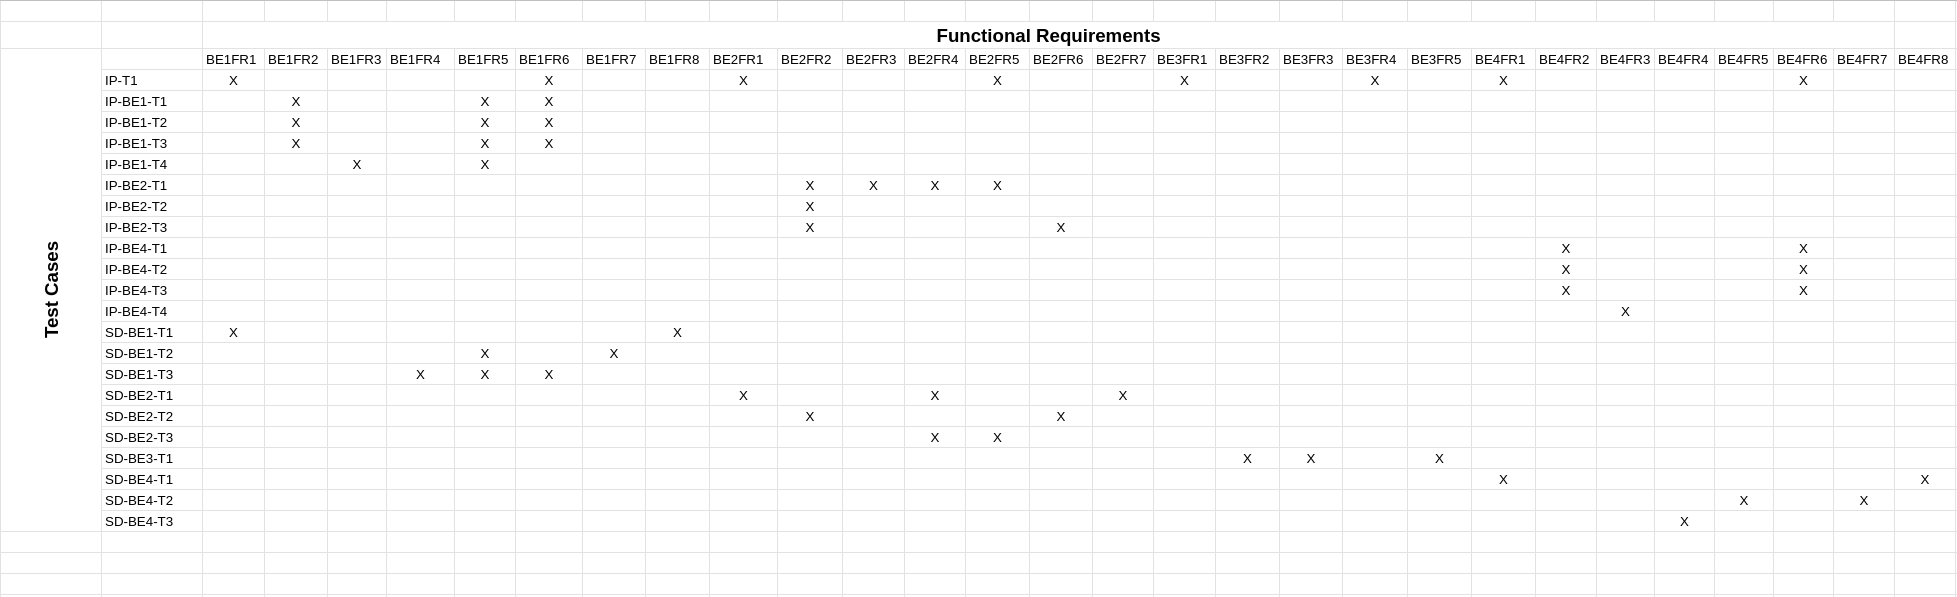
\includegraphics[scale=0.25, angle=90]{FR-1.png}
    \caption{Traceability Matrix for Functional Requirements in BE1 to BE4}
    \label{fig:my_label}
\end{figure}

\begin{figure}[H]
    \centering
    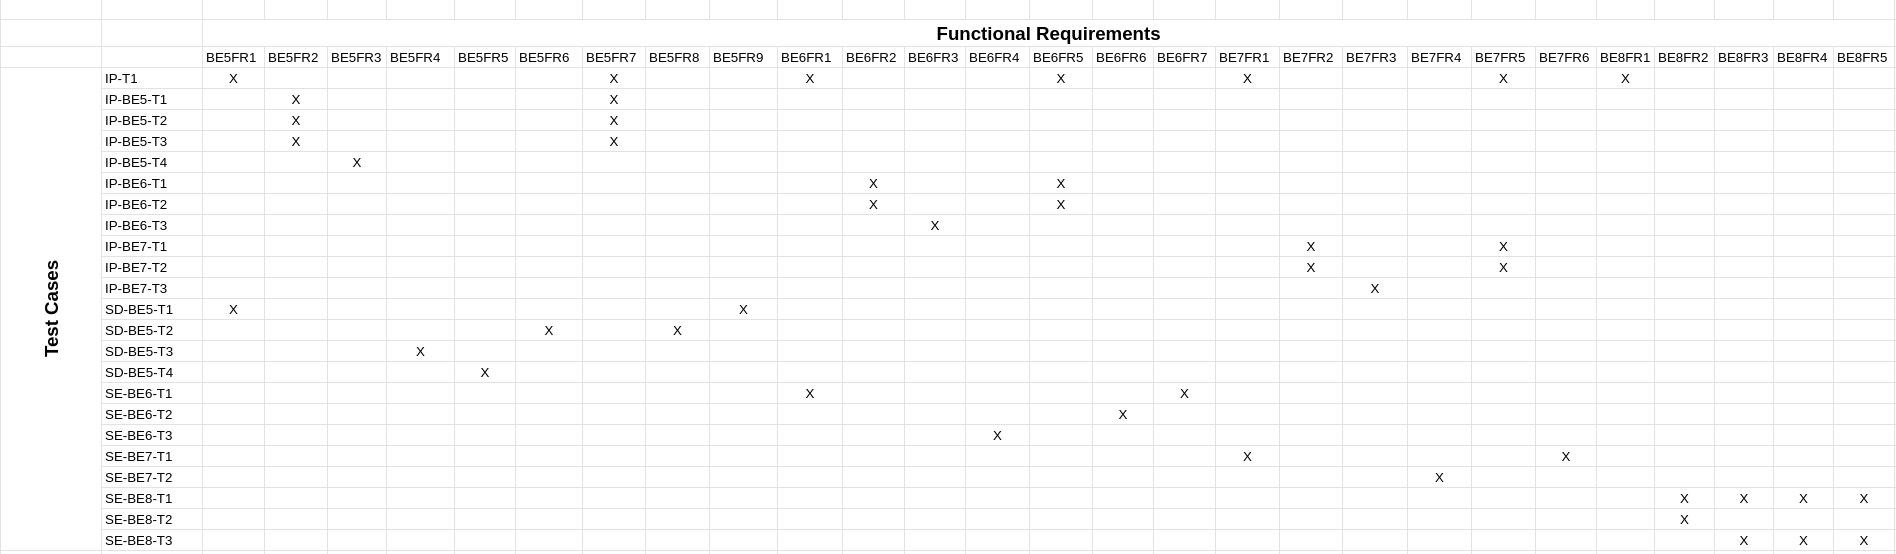
\includegraphics[scale=0.25, angle=90]{FR-2.png}
    \caption{Traceability Matrix for Functional Requirements in BE5 to BE8}
    \label{fig:my_label}
\end{figure}

\begin{figure}[H]
    \centering
    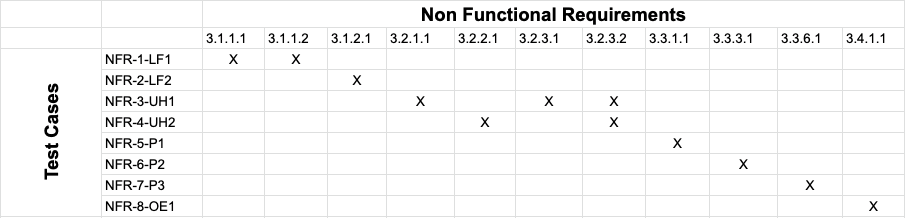
\includegraphics[scale=0.50, angle=90]{NFR.png}
    \caption{Traceability Matrix for Nonfunctional Requirements in NFR-1 to NFR-8}
    \label{fig:my_label}
\end{figure}

\section{Tests for Proof of Concept}

Our proof of concept demo implemented a good amount of the functional requirements related to creating a \textbf{table}, inserting \textbf{record}s, searching for \textbf{record}s and listing all \textbf{table}s. Most of the tests for the proof of concept were manual integration tests as follows:

\subsection{System-Wide Testing}
		
\begin{enumerate}

\item{POC-T1\\}

Type: Functional, Dynamic, Manual
					
Initial State: The \textbf{command line} interface is initialized and waiting for user input
					
Input: A create \textbf{table} statement with missing fields
					
Output: Appropriate error for missing fields is returned to the user
					
How test will be performed: This test was performed manually by supplying incorrect create \textbf{table} statements missing \textbf{primary key}s or \textbf{table} names and the output was manually verified to return the correct error statement.
					
\item{POC-T2\\}

Type: Functional, Dynamic, Manual
					
Initial State: The \textbf{command line} interface is initialized and waiting for user input
					
Input: A insert tuple statement with missing fields
					
Output: Appropriate error for missing fields is returned to the user
					
How test will be performed: This test was performed manually by supplying incorrect insert tuple statements missing \textbf{table} name or \textbf{column} data and the output was manually verified to return the correct error statement. 

\item{POC-T3\\}

Type: Functional, Dynamic, Manual
					
Initial State: The \textbf{command line} interface is initialized and waiting for user input
					
Input: A create \textbf{table} statement without syntactic errors and a unique \textbf{table} name, followed by a list \textbf{table}s statement
					
Output: The newly created \textbf{table} should be displayed in the output of the list \textbf{table}s statement
					
How test will be performed: This test was performed manually a correct create \textbf{table} statement and then supplying a list \textbf{table} statement to observe the newly created \textbf{table} in the output.

\item{POC-T4\\}

Type: Functional, Dynamic, Manual
					
Initial State: The \textbf{command line} interface is initialized, waiting for user input and the \textbf{database} has \textbf{table}s inserted
					
Input: A insert \textbf{record} statement without syntactic errors and a unique \textbf{table} name, followed by a select statement
					
Output: The newly inserted \textbf{record} should be displayed in the output of the select statement statement
					
How test will be performed: This test was performed manually a correct insert \textbf{record} statement and then running a select query on the \textbf{table} to observe the newly created \textbf{record} in the output. 

\end{enumerate}
	
\section{Comparison to Existing Implementation}	
GoDBMS is a simpler implementation of a DBMS as compared to SimpleDB. It is implemented in Go rather than Java. Memory usage has so far been optimized by using pointers instead of implicit objects. Only basic data types string and integer are supported in GoDBMS as compared to the larger range of types allowed in SimpleDB. A simple CLI has also been implemented instead of requiring a third party software to pass queries. Concurrency and message passing remains to be implemented. Overall however, GoDBMS preserves the basic functionality of SimpleDB.
				
\section{Unit Testing Plan}

		
\subsection{Unit testing of internal functions}
Unit testing on internal functions will be performed using Go's built-in standard library for testing called testing package. Tests for each unit/function are written in the form of individual testing functions, in which the result assigned the value of a function call with predefined test case parameters. The result is then compared to the manually determined expected result with comparator logic. Using the Go testing package library, all the test functions in the test driver will execute when the go test command is ran, and the \textbf{command line} will display a PASS or FAIL status for each test as well as its runtime.
		
\subsection{Unit testing of output files}	
Output and log files are not testable in this implementation.

\bibliographystyle{plainnat}

\bibliography{SRS}

\newpage

\section{Appendix}

\subsection{Symbolic Parameters}

The definition of the test cases will call for SYMBOLIC\_CONSTANTS.
Their values are defined in this section for easy maintenance.\\

\noindent $\hypertarget{time}{RESPONSE\_TIME}$ = 5 seconds

\subsection{Usability Survey Questions?}

\begin{enumerate}
    \item On a scale of 1 to 10, how comfortable were you using the \textbf{database} on the \textbf{command line} interface compared to other \textbf{database}s on the \textbf{command line} interface like IBM DB2?
    
    \item Were they any visual disturbances or inconveniences when starting up the \textbf{database}? 
    
    \item On a scale of 1 to 10, how intuitive was the user experience when you first started using the \textbf{database}
    
    \item Were there any confusions with the prompts or errors that were given by the \textbf{database}?
    
\end{enumerate}

\end{document}
